\section{Generalization to Multiple Tasks}\label{sec:generalize}

We further implement SCSP in different scenarios to evaluate its generalization. Using multi-contact tasks and long-horizon tasks as examples, we demonstrate that SCSP can perform \rev{online contact selection} and execute more complex manipulation tasks on more underactuated objects.

\subsection{Case Study I: Multi-Contact Task}

SCSP can be easily extended to multi-contact tasks. We illustrate the generalization of SCSP with following example:
\subsubsection{Soccer Dribbling}
We use a soccer dribbling task to demonstrate \rev{the performance of SCSP in dynamic scenarios}. In this task, SCSP plans contact with the ball using one of the two feet and drives it toward the goal through multi-contact manipulation. The main challenges lie in the highly dynamic behavior of the ball, which makes stable and sustained contact difficult, and in coordinating the two feet effectively. We read the ball position $\boldsymbol{p}_k$ and estimate its velocity $\boldsymbol{v}_k$ from the simulation using a Kalman filter. The 3D model of the ball is then input to the SCSP to compute the actions $\boldsymbol{u} \in \mathbb{R}^{2\times 4}$ for both feet, where the control vector for each foot is $\left [ x,y,z,\theta_{\mathrm{yaw}} \right ] $. We define activation triggers separately for the left and right feet: using the midpoint between both feet as the center, the space is divided into left and right half-spaces. When $\boldsymbol{x}_k$ appears in a half-space, the corresponding left or right foot is activated. Additionally, workspace constraints (represented as semi-transparent cubes) are imposed on each foot to prevent singular gait patterns. The number of CSO sampling points is set to $n_s=70$, and points close to the ground $\left \{ p_i\in\mathcal{I}_{\text{obj}} \ | \ z_i < 0.02\mathrm{m}  \right \}$ are masked out. We randomly selected 10 goal positions for the soccer ball, and SCSP continuously controlled the robot’s feet to dribble the ball to each target, achieving a 100\% success rate. The experimental results are shown in Fig. \ref{fig:soccer}. This experiment serves as a toy example, simulating the approaching and contact phases in humanoid soccer dribbling. In the future, we plan to extend SCSP to more complex motion planners to realize a more complete demonstration \cite{yin2025visualmimic, kong2026learning}.
\begin{figure}[!t]
 \centerline{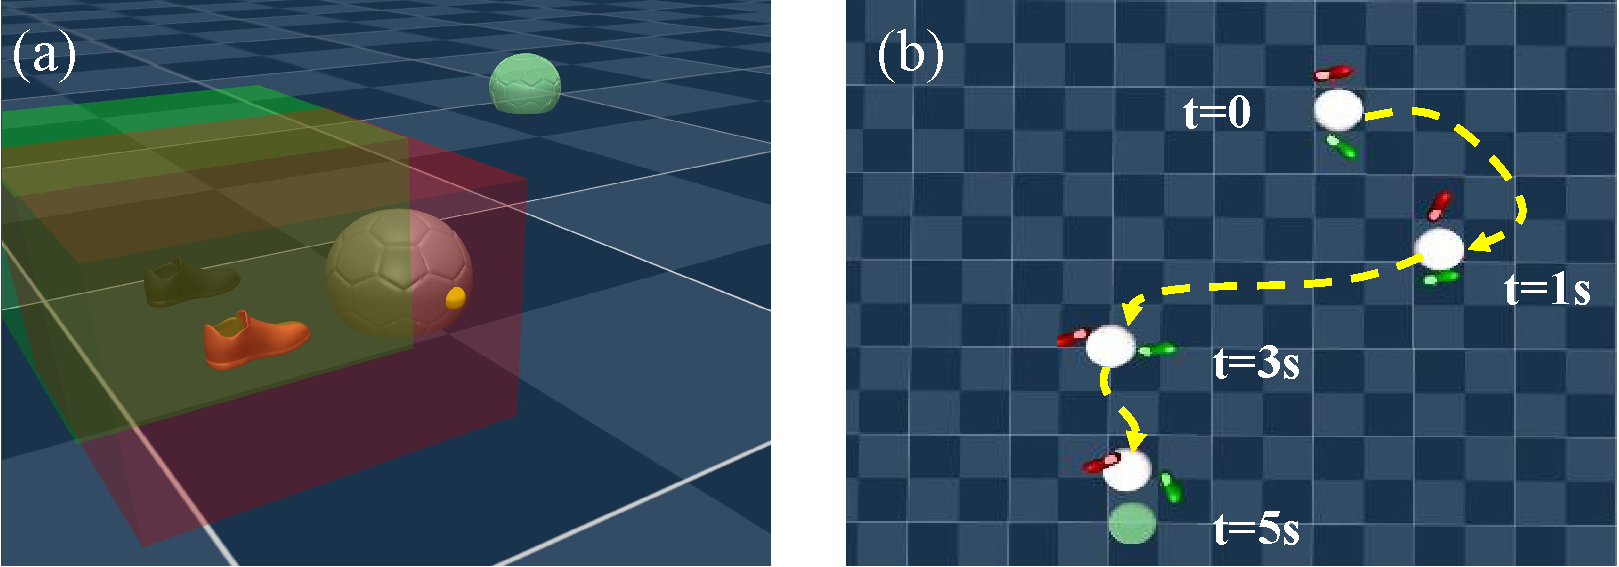
\includegraphics[width=\columnwidth]{figures/soccer2.pdf}}
\caption{Soccer dribbling task. (a) Experiment setup. The task is to kick the soccer to the target (translucent). Red and green cubes show footworkspaces, and the yellow point indicates CSO-planned contact locations. (b) Gribbling trajectory.}
\label{fig:soccer}
\end{figure}
\subsubsection{Tilted Pushing} 

SCSP can be extended to manipulation tasks in uneven environments, such as tilted pushing. Stable object poses on a slope are inherently fragile, requiring accurate contact location selection and online replanning. We compare open-loop methods, which plan a contact sequence offline, with SCSP, which replans online during execution. As the baseline, we use STOCS-3D to compute an offline sequence of contact locations and contact forces, and execute this sequence using our CPO. Experiments are conducted in \texttt{IsaacGym} with a 15$^\circ$ slope and a friction coefficient of 0.1. For SCSP, we set $w_{\text{stab}}=0$ and $\hat{\lambda}^n_{\text{max}}=0.5$, while keeping all other parameters the same as in Section~\ref{sec:robot_manipulation}. We selected the teapot and duck (used in previous experiments) and randomly set 10 stable poses on the slope as goal poses, and pushed and rotated the objects from below to reach these goals. The results in Table~\ref{tab:generalization_tasks_result} and Fig.~\ref{fig:tilted_push} show that the real-time replanning capability of SCSP provides substantially better robustness.

\begin{figure}[!t]
 \centerline{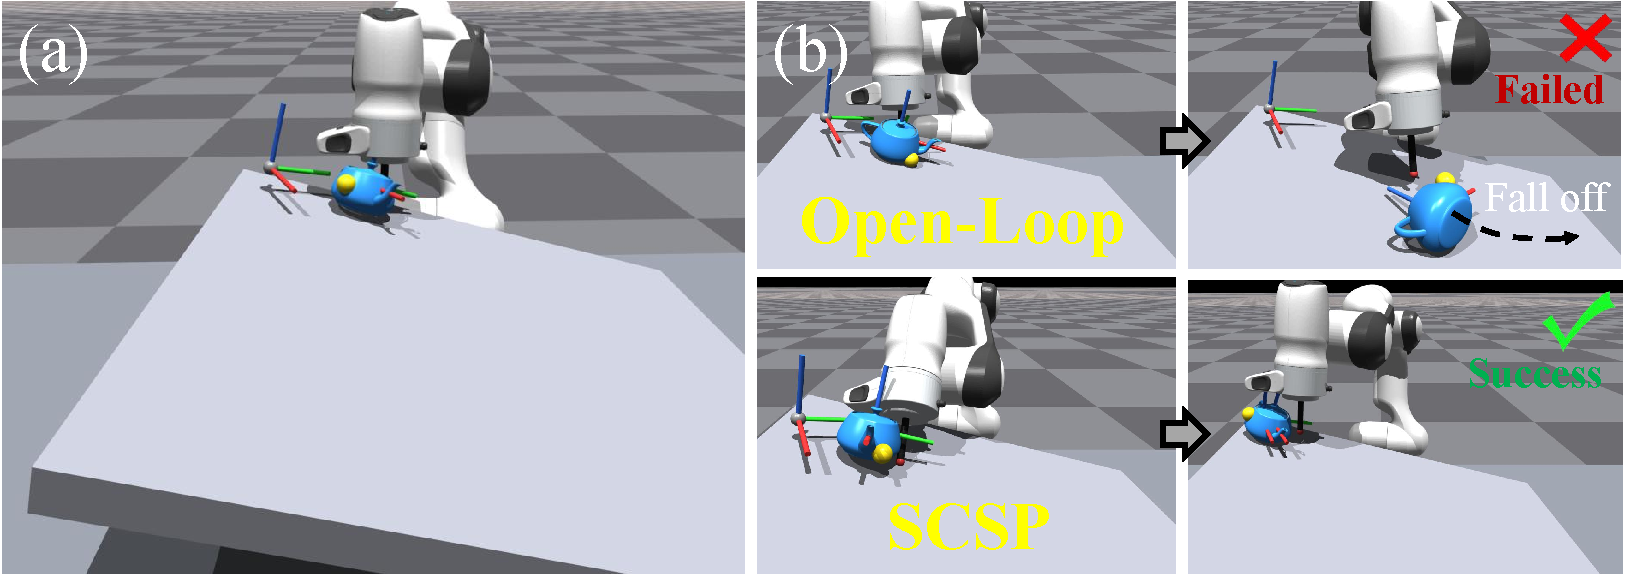
\includegraphics[width=\columnwidth]{figures/tilted_pushing.pdf}}
\caption{Experiment setup. The task is to push an object on a surface tilted at 15$^\circ$. (a) The open-loop method fails when execution errors occur, causing the teapot to fall off the tilted surface. (b) SCSP can replan online and thus successfully complete the dynamic task.}\label{fig:tilted_push}
\end{figure}
\subsubsection{Grasping \& Dexterous Manipulation} 
SCSP can also be applied to predict grasping poses, such as bimanual grasping and multi-finger grasping. Following \cite{lin2026bidexgrasp}, we use the Grasp Wrench Boundary (GWB) \cite{borst2004grasp} to select grasping regions and identify the top-K pairs of potential valid regions for grasping. Subsequently, sampling of the candidate set $\mathcal{I}_{\text{obj}}$ is performed within these regions. The objective of the CSO inner loop optimization is then transformed to force closure:
\begin{equation}\label{equ:force_closure}
    \begin{aligned}
\min_{\boldsymbol{\hat{\lambda}}_r \in \mathcal{K}}
\quad &
\sum_{j=1}^{N_d} \left\| \xi \boldsymbol{w}^{(j)} - \boldsymbol{J}_o \boldsymbol{\hat{\lambda}}_r^{(j)} \right\|_2^2
\;+\;
w_{\lambda} \sum_{j=1}^{n_d} \left\| \boldsymbol{\hat{\lambda}}_r^{(j)} \right\|_2^2 \\
\text{s.t.}\quad
& \sum_{i=1}^{K} \hat{\lambda}_r^{(j),n} \ge \zeta, \ 
\forall j=1,\dots,n_d .
\end{aligned}
\end{equation}
where $n_c$ is the number of robot contact points, $n_d$ denotes the number of sampled disturbance wrenches, $\boldsymbol{w}^{(j)} \in \mathbb{R}^6$ represents the $j$-th disturbance wrench. $\boldsymbol{\lambda}_r^{(j)}$ denotes the robot contact force corresponding to disturbance $\boldsymbol{w}^{(j)}$. $\xi$ is the disturbance scaling factor, $\zeta$ the minimum total normal force required to maintain an active grasp and $w_{\lambda}=0.1$. During each rollout, the CSO in SCSP solves \eqref{equ:force_closure} for the nearest points $\boldsymbol{p}_{\text{near}}^i$ to the robot end-effector or Allegro fingers additional to the top 5 pairs of potential grasping pairs, thereby searching for grasping poses online. We use an open-loop baseline that computes the optimal grasping locations offline using CSO and executes them online with CPO for comparison. For bi-manual and multi-finger grasping, we selected five objects each, placed them on a pedestal (black), randomly perturbed their yaw angles $\theta_{\text{yaw}}$ and scaled their sizes by a random factor $\varsigma \in \left \{ 0.5,1,1.5,2 \right \} $, conducting 20 trials for each task. The results are shown in Table~\ref{tab:generalization_tasks_result} and Fig.~\ref{fig:grasping}. SCSP achieves a higher success rate than the baseline in these trials; however, it fails on some objects with complex geometry because automatic convexification of the collision mesh by \texttt{MuJoCo}.
\begin{figure}[!t]
 \centerline{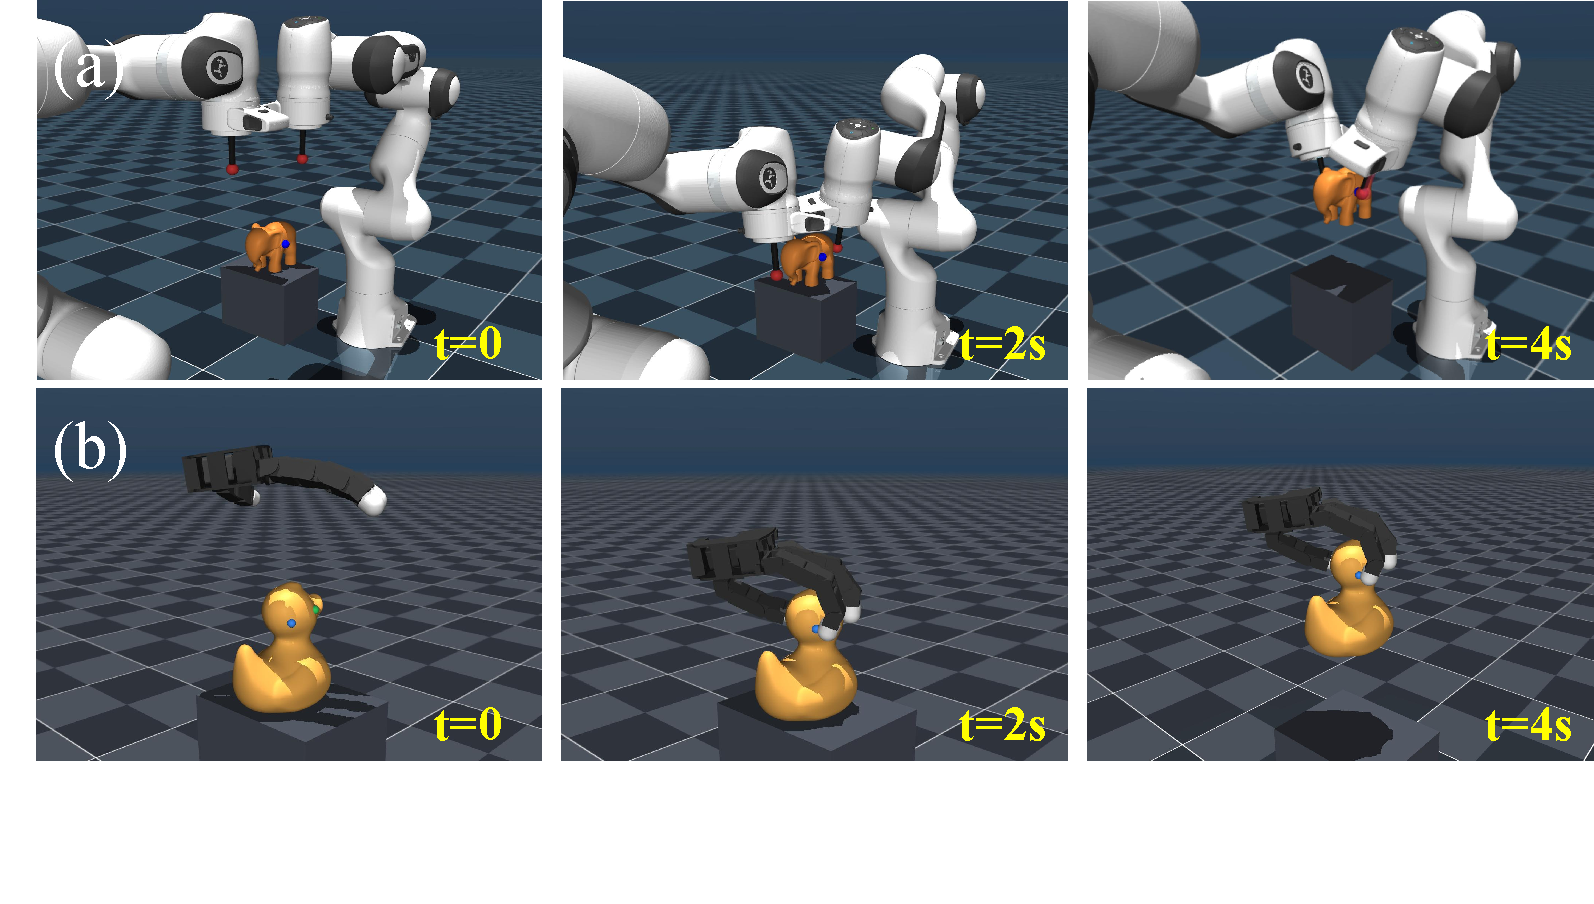
\includegraphics[width=\columnwidth]{figures/grasping.pdf}}
\caption{Snapshots of the multi-contact grasping tasks. (a) Bi-manual grasping of an elephant with the size scaling factor $\varsigma=1$. (b) Multi-finger grasping of a duck with $\varsigma=1.5$.}
\label{fig:grasping}
\end{figure}
\subsection{Case Study II: Articulated Object Manipulation}
\rev{SCSP uses active contact selection to perform articulated object manipulation. We evaluate this capability on a drawer and a microwave door, which require sequential contact interactions.} The tasks are to pull the drawer to a target displacement and to open the microwave door to a target angle. In both tasks, the object is semantically segmented into different parts, such as handles, while non-manipulable parts are excluded. For the drawer, we directly compute the final pulled-out pose as the goal pose. For the microwave, which involves rotational motion, we set the goal pose of each rollout as the \texttt{SLERP} interpolation between the current state and the desired door state. The parameter and cost settings of SCSP are the same as those in Section~\ref{sec:robot_manipulation}, with $w_{\text{stab}}=0$. The solver for CPO is an MPPI-based motion planner~\cite{bhardwaj2022storm}. As a baseline, we use an open-loop method that plans the contact sequence offline using CSO and executes it online with CPO, in order to demonstrate the effectiveness of online contact selection. We randomly perturbed the distance and yaw angle between the drawer or microwave and the Franka base by $\Delta d \in \left [ -0.1, 0.1 \right ] \mathrm{m}$ and $\Delta \theta_{\text{yaw}} \in \left [ -\frac{\pi}{4} , \frac{\pi}{4}  \right ]$ and conducted 10 trials for each object. The experimental results are shown in Fig.~\ref{fig:long_horizon}, Table~\ref{tab:generalization_tasks_result} and the \href{https://sites.google.com/view/scsp-robot}{website} videos. Although the success rates are comparable, the open-loop method cannot handle certain execution errors, such as contact slippage or the robot approaching singular configurations.
\begin{figure}[!t]
 \centerline{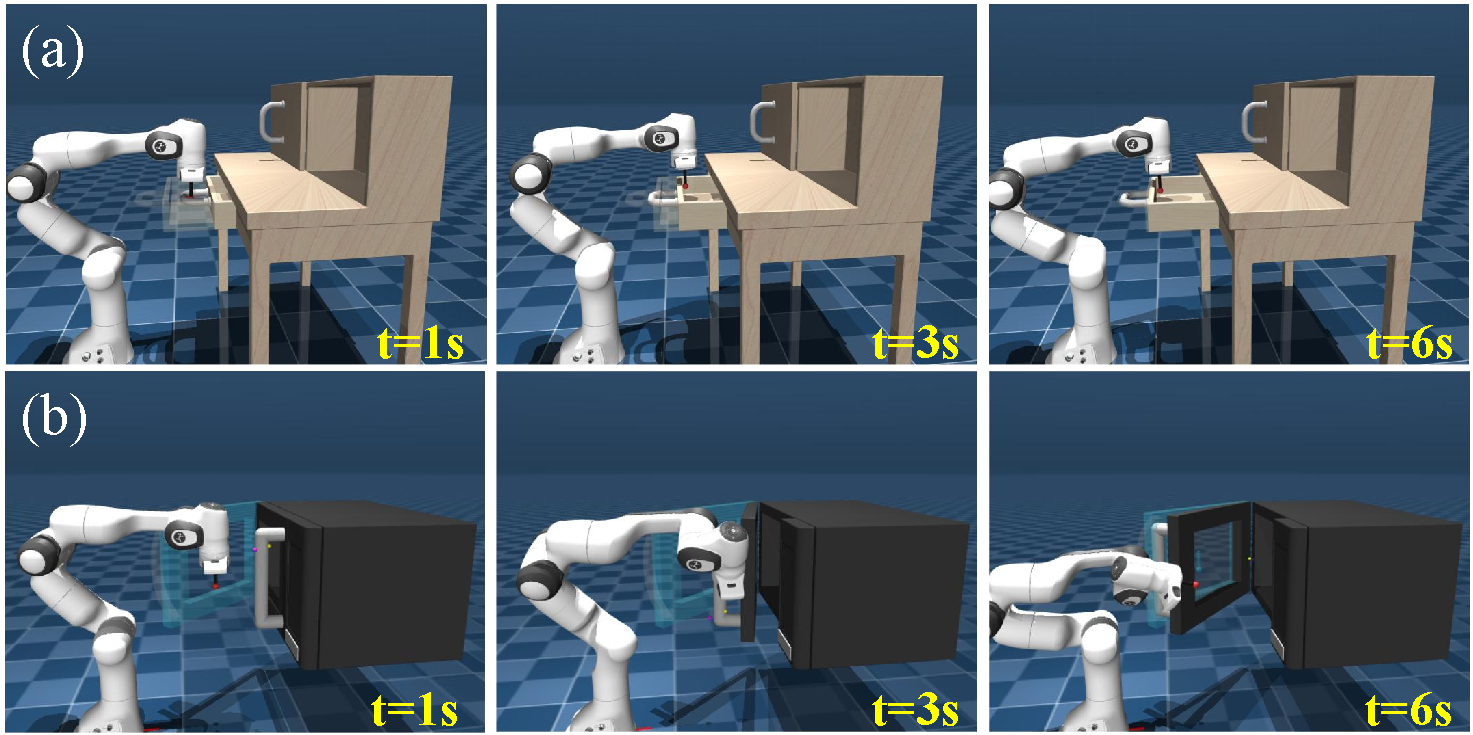
\includegraphics[width=\columnwidth]{figures/long-horizon.pdf}}
\caption{Snapshots of long-horizon tasks. Given only the target pose of the object, SCSP performs online reasoning and selects appropriate contact locations to accomplish the task. (a) Opening a drawer. (b) Opening the microwave door.}
\label{fig:long_horizon}
\end{figure}

\begin{table*}[t]
\centering
\caption{Success trials across different tasks.}
\label{tab:generalization_tasks_result}
\setlength{\tabcolsep}{5pt}
\begin{tabular*}{\textwidth}{@{\extracolsep{\fill}} lcccccccccc}
\toprule
\textbf{Metric}
& \multicolumn{2}{c}{\textbf{Soccer Dribbling}}
& \multicolumn{2}{c}{\textbf{Tilted Pushing}}
& \multicolumn{2}{c}{\textbf{Bi-Manual Grasping}}
& \multicolumn{2}{c}{\textbf{Multi-finger Grasping}}
& \multicolumn{2}{c}{\textbf{Long-horizon Tasks}} \\
\cmidrule(lr){2-3}
\cmidrule(lr){4-5}
\cmidrule(lr){6-7}
\cmidrule(lr){8-9}
\cmidrule(lr){10-11}
& \textbf{Open-Loop}
& \textbf{SCSP}
& \textbf{Open-Loop}
& \textbf{SCSP}
& \textbf{Open-Loop}
& \textbf{SCSP}
& \textbf{Open-Loop}
& \textbf{SCSP}
& \textbf{Open-Loop}
& \textbf{SCSP} \\
\midrule
\textbf{Success Trials}
& /
& \textbf{10/10}
& 0/20
& \textbf{18/20}
& 0/20
& \textbf{15/20}
& 15/20
& \textbf{16/20}
& 15/20
& \textbf{20/20} \\
\bottomrule
\end{tabular*}
\end{table*}



